\chapter{Infinite Prandtl number Thermal Convection}
\label{cha:thermal-convection}

\section{Problem Overview}
\label{sec:convection_problem-formulation}

A model multi-physics  problem in Solid Earth Sciences is the solution of
infinite Prandtl number thermal convection, which couples Stokes
Equation (Chapter \ref{cha:stokes-equation}) for flow of a highly
viscous fluid to an advection-diffusion
equation for evolution of temperature, i.e.
\begin{align}
-\div\eta(\grad\vec{v} + \grad\vec{v}^{T}) + \grad p & = T\vec{k} \label{eq:rbconvv}\\ 
\div \vec{v} &= 0  \label{eq:rbconvp}\\
  \ppt{T} + \vec{v}\cdot\grad T - \frac{1}{\Ra}\nabla^2 T &= 0 \label{eq:rbconvT}
\end{align}
$\vec{v}$, $p$ are the dimensionless velocity and pressure, $T$ is
dimensionless temperature, and $\eta$ is dimensionless viscosity which
can be constant ($\eta=1$) or a function of $T$, $\vec{v}$ and/or $p$.
\begin{displaymath}
  \Ra = \frac{\rho g \alpha \Delta T h^{3}}{\eta_{0}\kappa}
\end{displaymath}
is the Rayleigh number for a layer of depth $h$, temperature
difference $\Delta T$ and reference viscosity $\eta_{0}$. 
% Do we need this next bit? 
% PvK: yes, useful since most geodynamicists use the other scaling.
Note, \eqref{eq:rbconvv}--\eqref{eq:rbconvT} scale velocity by
$\vec{v}=v_0\vec{v}'$ with
\begin{equation}
  \label{eq:6}
  v_0 = \frac{\rho g\alpha\Delta T h^{2}}{\eta_0}
\end{equation}
which is roughly the Stokes rise velocity of a buoyant blob of size $h$, rather than the
more standard ``diffusion velocity'' $v_0=\kappa/h$. This
scaling puts $1/\Ra$ in the diffusion term in \eqref{eq:rbconvT}, rather
than multiplying $T$ in \eqref{eq:rbconvv}. For large $\Ra$, \eqref{eq:rbconvT}
is dominantly advective with narrow diffusive boundary layers. 

Thermal convection is a good example of a multi-physics 
problem as it describes the coupled interactions of three fields;
velocity, pressure and temperature. Equations
\eqref{eq:rbconvv}--\eqref{eq:rbconvp} are  Stokes equations for incompressible viscous flow and are linear in $\vec{v}$ and $p$ if $T$ is
known and $\eta$ is independent of velocity.  Likewise,
\eqref{eq:rbconvT} is an advection-diffusion equation for $T$ and
appears linear in $T$ if $\vec{v}$ is known.   When all three fields are unknown then the coupled system $\vec{u}=\left(\vec{v}, p,
T\right)$ is non-linear because the velocity is a function of temperature and vice versa.  Adding additional coupling through more
complex rheologies, $\eta\left(T,\vec{v},p\right)$, only increases the
non-linearity of the system. These problems can be solved using either
Newton's method (N) or a Picard splitting scheme (P), which both can
be implemented in \TF{}.


\subsection{Variational forms}
\label{sec:variational-forms}

For this tutorial, we will reuse the setup for  Stokes using
``Taylor-Hood'' elements from 
Chapter \ref{cha:stokes-equation} and add to it an energy equation for
Temperature using quadratic $P_{2}$ elements. To solve the energy
equation, we start by discretizing the time derivative
using finite differences as
\begin{displaymath}
  \ppt{T}\approx(T_{i} - T_{n})/\Delta t
\end{displaymath}
where $T_{i}$ is our current estimate of the value of temperature at the new
time and $T_{n}$ is temperature at the previous time. We use a
$\theta$ scheme  for time-integration of the advection-diffusion
equation.  Multiplying by appropriate test functions and integrating by parts, the
variational form of the non-linear problem can be written
\begin{quote}
  \fbox{\parbox{.9\textwidth}{Find $\vec{u}\in \fspace$ such that
      \begin{equation}
         F(\vec{u};\vec{u}_{t}) =0 
      \end{equation}
  for all test functions $\vec{u}_{t}=(\vec{v}_{t},p_{t},T_{t}) \in\fspace$.}}
\end{quote}
 where $F(\vec{u};\vec{u}_{t}) = F_{\vec{v}} + F_{p} + F_{T}$ with
\begin{align}
         F_{\vec{v}} =  & \int_\Omega \left[\dot{\epsilon}(\vec{v}_{t}):
             2\eta \dot{\epsilon}(\vec{v}_{i}) -
             p_{i}\div\vec{v}_t  - T_{i}\vec{v}_{t} \cdot\vec{k} \right]d\vec{x}  \\
 F_{p} =& -\int_\Omega p_t\div\vec{v}_{i} d\vec{x}\\
F_{T}  = &\int_\Omega \left[ T_t\left(T_{i} - T_{n} + \Delta t\vec{v}_{\theta}\cdot\nabla T_{\theta}\right) +\frac{\Delta t}{\Ra}\nabla
T_t \cdot\nabla T_\theta \right]d\vec{x} \label{eq:26}\\
\nonumber \\
  F = & F_{\vec{v}} + F_{p} + F_{T} 
\end{align}
where \begin{equation}
  \label{eq:19}
  \dot{\epsilon}(\vec{v}) = \frac{1}{2}
  \left(
\grad\vec{v} + \grad\vec{v}^{T}
  \right)
\end{equation} is the strain-rate tensor and 
\begin{align*}
  T_{\theta} = & (1-\theta)T_{n} + \theta T_{i}\\
  \vec{v}_{\theta} = & (1-\theta)\vec{v}_{n} + \theta \vec{v}_{i}
\end{align*}
are $\theta-$weighted variables such that $\theta=0$ is a fully
explicit first order Euler scheme, $\theta = 1$ is a fully implicit
backwards Euler scheme and $\theta = 1/2$ is a second-order,
Crank-Nicolson (trapezoidal) scheme.  Here we use $\theta=1/2$.
For a specific choice of a mixed finite element space for $\vec{u}_{i}$ and
$\vec{u}_{t}$, \eqref{eq:4} assembles into a vector which is the
discrete residual of the full system. 

The weak form of the residual in UFL looks quite similar
\begin{lstlisting}[style=UFL]
T_theta = theta*T_i + (1.-theta)*T_n
v_theta = theta*v_i + (1.-theta)*v_n 

Fv = (inner(sym(grad(v_t)),2.*eta*sym(grad(v_i)))
    - p_i*div(v_t) - T_i*v_t[1])*dx  
Fp = -p_t*div(v_i)*dx 
FT = (T_t*(T_i - T_n  + dt*inner(v_theta, grad(T_theta))) 
    + dt/Ra*inner(grad(T_t), grad(T_theta)))*dx 

F =  Fv + Fp +FT
\end{lstlisting}

For the simplest
isoviscous problem ($\eta=1$) the inner linear solve in a Newton solver
$(J\left(\vec{u}_i\right)\vec{\delta u}_i=-F\left(\vec{u}_i\right))$ looks like
\begin{equation}
  \label{eq:7}
  \left[
\begin{array}{ccc}
  K & G  & M \\
  G^{T} & 0 & 0 \\
  B & 0 & A \\ 
  \end{array}
  \right]
  \left[
    \begin{array}{c}
      \vec{\delta v} \\
      \delta p \\
      \delta T \\
    \end{array}
  \right] = -\left[
    \begin{array}{c}
      F_{\vec{v}}\\
      F_{p}\\
      F_{T}\\
    \end{array}
  \right]
\end{equation}
where the upper $2\times2$ block
\begin{displaymath}
     \left[
\begin{array}{cc}
  K & G  \\
  G^{T} & 0 \\
  \end{array}
  \right]
\end{displaymath}
is the discrete form of the Stokes equation, 
$M$ is a (mixed) mass matrix for buoyancy, $B(T_i)$ contains the
coupling between velocity and temperature and $A(\vec{v}_i)$ is the standard
advection-diffusion operator.  


There are a variety of benchmark problems for basic thermal
convection. As the simplest example, we will begin with the isoviscous
problem 1a described in Blankenbach et. al
\cite{blankenbach_benchmark_1989}, which solves for isoviscous thermal
convection in a unit-square domain with boundary conditions
\begin{align}
  \label{eq:rbconvBCs}
  T(x,0) = 1 &  \quad T(x,1) = 0\\
  \ppx{T}(0,z)=0 &  \quad\ppx{T}(1,z)=0\\
  \vec{v}\cdot\vec{n} = 0 & \quad \sigma\cdot\vec{n}= \vec{0} \quad\text{on } \partial\Omega 
\end{align}
where $\sigma = 2\eta \dot{\epsilon}(\vec{v})-pI$ is the stress tensor
(free stress boundary conditions) %check this
and $\Ra=10^{4}$.  While this problem admits a steady state solution,
we will calculate a fully time-dependent, time-accurate solution with
initial condition
\begin{displaymath}
  T(x,0) = 1 - z + 0.2\cos(\pi x)\sin(\pi z)
\end{displaymath}
to which will set up a steady cell rotating clock-wise.
\pagebreak{}
\section{Solution using \TF}
\label{sec:solution-using-tf}

To set this problem up in \TF{}, we will reuse a large amount of the
work from our Stoke's MMS solutions but extend it to solve the
time-dependent problem.  The principal changes will be
\begin{itemize}
\setlength{\itemsep}{-.1em}
\item Set the domain to  $[0,1]\times[0,1]$ 
\item Add timestepping options including a simple adaptive time stepper.
\item Adding an additional scalar field $T\in P_{2}$ with initial and
  boundary conditions appropriate  to the system
\item Modifying the non-linear residual to the above UFL
\item Modify the solver to handle an additional field (if using
  fieldsplit block-preconditioners)
\item Adjust appropriate monitors and diagnostics
\end{itemize}

A fully worked out \texttt{tfml} file for this problem using a direct
solver %along with a script to perform a basic convergence test
can be found in
\texttt{\$TF\_HOME/share/terraferma/tutorials/thermalconvection/isoviscous/newton\_exact/convection.tfml}.  The
solution is shown in Figure \ref{fig:convection1a}.   


\begin{figure}[htbp!]
  \centering
  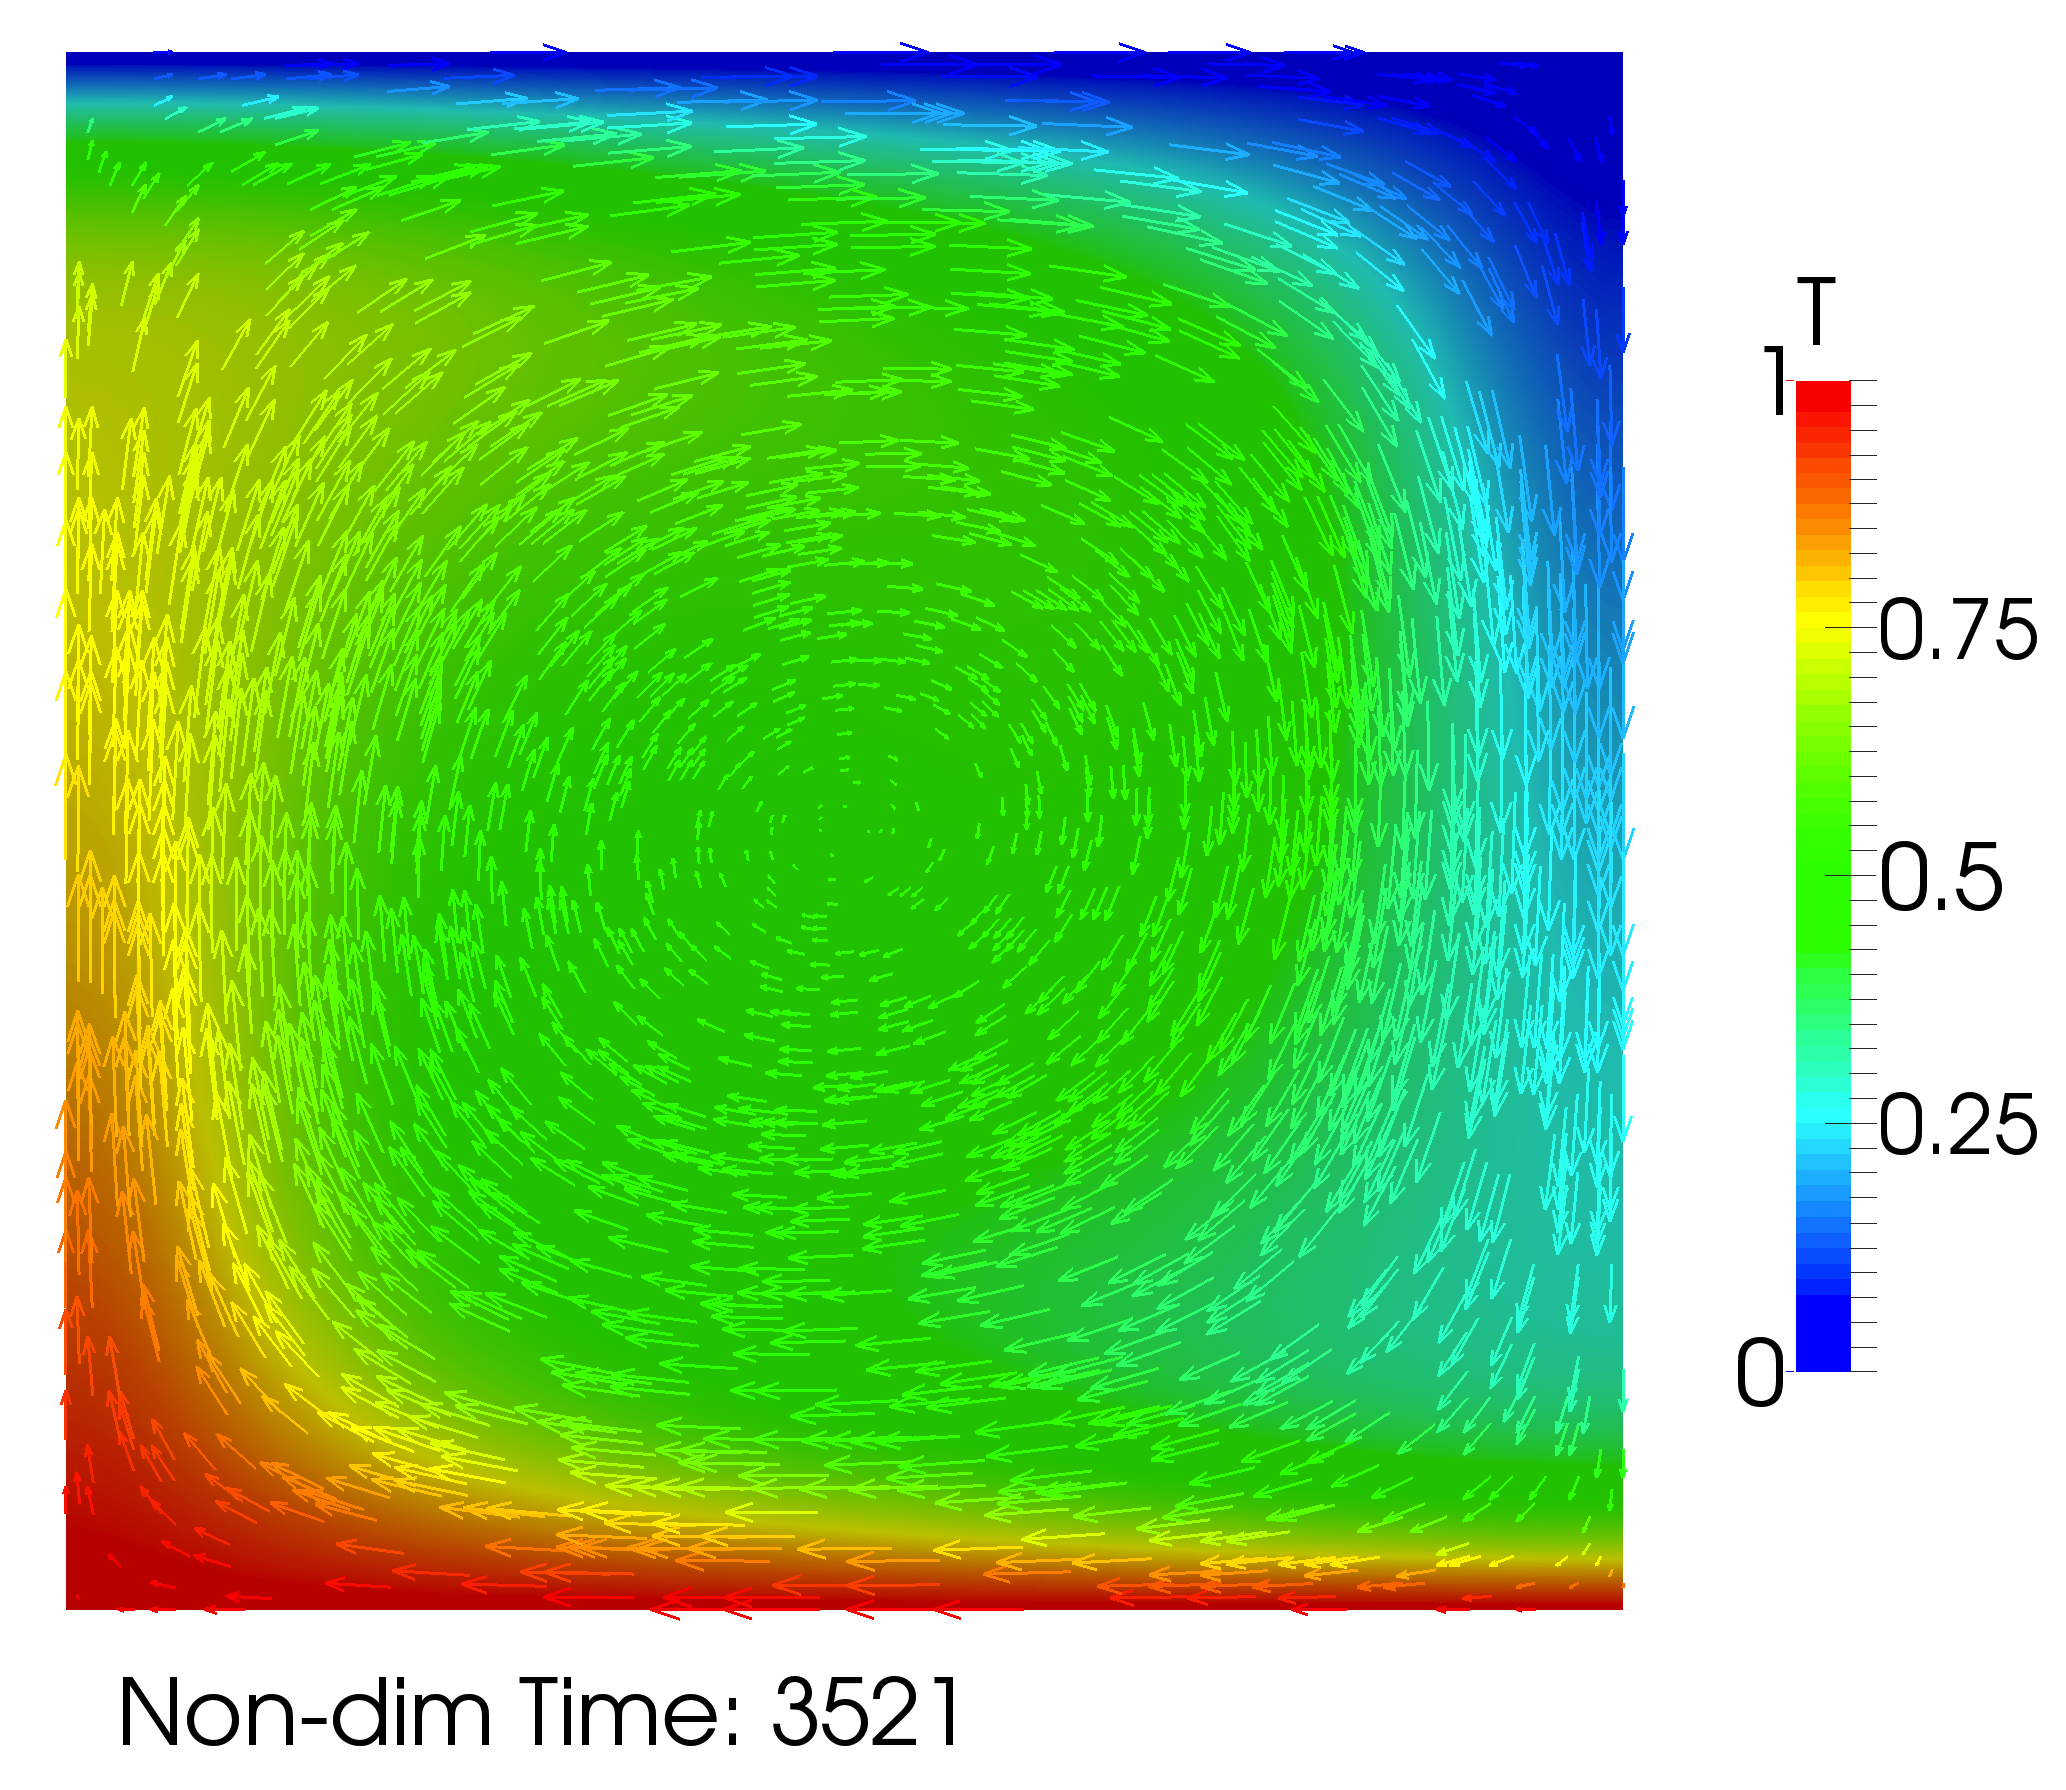
\includegraphics[width=.7\textwidth]{figures/convection_Tv.png}
  \caption{Steady state solution of a simple isoviscous thermal
    convection problem Blankenbach 1a
    \cite{blankenbach_benchmark_1989} ($\Ra=10^{4}$). Color field
    shows dimensionless Temperature with the velocity field shown with
    arrows.}
  \label{fig:convection1a}
\end{figure}

\pagebreak{}

In more detail, the specific steps required to modify the Stokes mms
problem to solve thermal convection are as follows.
\begin{steps}{Step}
\item Make a new tfml file
  \begin{lstlisting}[style=Bash]
$ mkdir myconvection
$ chdir myconvection
$ cp $TF_HOME/share/terraferma/tutorials/stokes/isoviscous/mms/mms_direct/stokes.tfml convection.tfml
$ diamond convection.tfml &
  \end{lstlisting}%$
\item \textbf{Change the geometry:} Under \texttt{geometry->Mesh},
  \begin{steps}{step}

  \item Set rectangle bounds to unitsquare $[0,1]\times[0,1]$. (or
    change mesh to UnitSquare).
  \item increase \texttt{number\_cells} to $64\times64$
  \end{steps}
\item \textbf{Change io parameters}
  \begin{steps}{step}
  \item Change \texttt{output\_base\_name} to \texttt{convection}
%  \item Change \texttt{visualization->element} to (P2DG)
  \item Add appropriate dump-periods for visualization and statistics
    output.  Under \texttt{dump\_periods} do the following
    \begin{itemize}
    \item Activate \texttt{visualization\_period} and set to
      100. (i.e. output paraview files every 100 dimensionless time units)
    \item Check and output statistics every 10 time steps. Activate
      \texttt{statistics\_period}, change it to
      \texttt{statistics\_period\_in\_timesteps}, and set it to 10
    \item Check for steady state stopping criterion every 10 time
      steps. Activate \texttt{steady\_state\_period} and change it to
      \texttt{steady\_state\_period\_in\_timesteps} and set it to 10
      (i.e. check every 10 time steps  whether the change in the solution from
      time-step to time-step is lower than the steady-state tolerance)
    \end{itemize}
  \end{steps}
\item \textbf{Add Time-stepping parameters}:
  \begin{steps}{step}
    \item Activate the \texttt{timestepping} tab and set the following
    \begin{itemize}
    \item \texttt{current\_time} = 0.0
    \item \texttt{finish\_time} = 1.e6
    \end{itemize}
    This will run for a dimensionless time of $10^{6}$ or until the
    solution has approached steady state (see below).
  \item \textbf{Set the time-step coefficient \texttt{dt}} Because we
    include the timestep $\Delta t$ explicitly in the form, we need to
    initialize it as a coefficient.  Unlike other coefficients, we do
    this in the Time-stepping tabs as we can add additional
    constraints such as adaptive time-stepping.
    \begin{itemize}
    \item\textbf{ Set the time-step ufl name.} Unfold\texttt{ coefficient(Timestep)} and set the
      \texttt{ufl\_symbol} to \texttt{dt}
    \item \textbf{Set the initial time-step value.}  The time step is
      of type \texttt{Constant}.  For a constant time-step just unfold the \texttt{type(Constant)} tab all the way to set
      the constant value to a fixed value.  Here however we will use
      adaptive time stepping which allows us to set the initial value
      to \textbf{0.0}. Inspection of Equation (\ref{eq:26}) shows that
      for \texttt{dt=0}, the problem reduces to a projection problem
      for $T_{i}$ that will simply set it to the initial condition at
      $t=0$, and then the Stoke's solver will solver for the $\vec{v}$
      and $p$ at the initial time.  After the first time-step, the
      adaptive time stepper will choose an appropriate value of
      \texttt{dt} based on a Courant condition.
    \end{itemize}
  \item \textbf{Set Adaptive Time-stepping parameters}. This problem
    will set a crude adaptive time-stepper based on a Courant number
    constraint.  In general, our constraints will
    scale with $\Delta t$, e.g. the Courant number can be considered a
    field
    \begin{displaymath}
      \alpha = \frac{\Delta t ||\vec{v}||}{h}
    \end{displaymath}
    where $h$ is a measure of the local cell-size.  Given a field
    calculated with the current time-step,  the time-stepper will
    return a modified time-step that keeps $\alpha$ to some maximum
    value (e.g. $\alpha=1$).  The actual Courant number will be calculated in a
    separate system described below.    Here we just inform TerraFERMA how the
    constraint will be implemented.  Do the following
    \begin{itemize}
    \item Activate the
    \texttt{adaptive} tab and add a \texttt{constraint} named
    \texttt{Courant}.
  \item Add the system name that calculates the constraint set
    \texttt{system = CourantNumber}
  \item Set the field or coefficient that is evaluated
    (i.e. \texttt{Field = CourantNumber}
  \item Set the maximum value of the constraint
    \texttt{requested\_maximum\_value = 2.}
  \item In addition you can set fields to determine how often the
    timestep check is called (\texttt{adapt\_period}) as well as the
    maximum amount of growth per time-step when the time-step is
    increasing.  More details on these parameters is given in the help
    windows in diamond.
    \end{itemize}
  \item \textbf{Set a steady state check:} We can also stop the
    time-loop when the change from time-step to time-step for any set
    of monitored fields drops below some tolerance.  To activate a
    steady state check
    \begin{itemize}
    \item Activate the \texttt{steady\_state} tab
    \item Set the tolerance to \texttt{1.e-9}
    \end{itemize}
    When we describe the fields below we have the option of adding
    them to the steady-state checker.
  \end{steps}
\item \textbf{Add a few global ufl parameters:}  Sometimes it is
  convenient to define a few ufl parameters that will be included in
  all forms.  Here we will just set the values of $\theta$ and
  $\theta_{v}$ that control the theta weightings for Temperature and
  Velocity and define the viscosity as constant (by putting the
  viscosity here, we can more easily modify it later to non-constant viscosity).  Do the following:
  \begin{itemize}
  \item under \texttt{global\_parameters} activate the \texttt{ufl} tab
  \item replace the (string) with the following ufl
    \begin{lstlisting}[style=UFL]
# theta weightings for Temperature and velocity
theta = 0.5
theta_v = 0.5

# scaled viscosity 
eta = 1.
    \end{lstlisting}

  \end{itemize}
\textbf{Caution:} Global ufl options should be used sparingly
  as any change to them will force a re-compile and a regeneration of
  all the ufl code.  To modify constants as run-time parameters, set
  them up as coefficients.
\item \textbf{Modify System Stokes to System Convection}
  \begin{steps}{step}
  \item \textbf{Change the system name} to  \texttt{Convection} (the \texttt{ufl\_symbol}
    remains the same, \texttt{us})
  \item \textbf{Modify Properties for Velocity}.  We will need two
    sets of boundary conditions to impose the no-flow boundaries (the
    free-stress conditions are imposed in the weak-forms), as well as
    cleaning up some of the diagnostics and setting the steady-state
    checkers.  Do the following
         \begin{steps}{do}
      \item \textbf{Set $v_{x}=0$ on the left and right boundaries}: remove (or
        edit) the existing \texttt{boundary\_condition} tab to have
        the following parameters
        \begin{itemize}
        \item \texttt{boundary\_condition} name=\texttt{LeftRight}
        \item \texttt{boundary\_ids} = 1 2
        \item \texttt{sub\_components} name = \texttt{vx}
        \item \texttt{components} = 0
        \item \texttt{type(Dirichlet)} constant = 0
        \end{itemize}
      \item \textbf{Set $v_{y}=0$ on the top and bottom boundaries}: Repeat (or use the copy paste function in diamond) to
        make a second boundary condition for the top and bottom
        boundaries
        \begin{itemize}
        \item \texttt{boundary\_condition} name=\texttt{TopBottom}
        \item \texttt{boundary\_ids} = 3 4
        \item \texttt{sub\_components} name = \texttt{vy}
        \item \texttt{components} = 1
        \item \texttt{type(Dirichlet)} constant = 0
        \end{itemize}
      \item \textbf{Delete the Functional} \texttt{L2NormErrorSquared}
      from \texttt{diagnostics $\rightarrow$ include\_in\_statistics}
    \item \textbf{Turn on steady-state checking} Activate the tab
      \texttt{include\_in\_steady\_state} and set the norm to be
      checked to \texttt{linf} (infinity norm)
      \end{steps}
    \item \textbf{Modify Properties for Pressure}
      \begin{itemize}
      \item Move the reference point to $[0.5, 0.5]$
      \item \textbf{Delete the Functional} \texttt{L2NormErrorSquared}  from \texttt{diagnostics $\rightarrow$ include\_in\_statistics}
      \item \textbf{Turn on steady-state checking} Activate the tab
      \texttt{include\_in\_steady\_state} and set the norm to be
      checked to \texttt{linf}
      \end{itemize}
    \item \textbf{Add a new Field and diagnostics for Temperature}.
      Activate a new field and set the following properties, BC's and IC's
      \begin{itemize}
      \item \texttt{name} = \texttt{Temperature}
      \item \texttt{ufl\_symbol} = T
      \item \textbf{Set properties of the \texttt{type(Function)}}
        \begin{steps}{do}
        \item set \texttt{rank(Scalar)}
        \item set \texttt{element(P2)}
        \item set the initial condition
          \begin{displaymath}
            T = 1. - y + 0.2\cos(\pi x)\sin(\pi y)
          \end{displaymath}
using the python Expression
\begin{lstlisting}[style=python]
def val(x):
  from math import sin, cos, pi
  return 1.-x[1] + 0.2*cos(x[0]*pi)*sin(x[1]*pi)
\end{lstlisting}
\item \textbf{Set the Dirichlet boundary condition on the top $T=0$}
  \begin{itemize}
  \item activate a new \texttt{boundary\_condition} tab and name it \texttt{Top}
\item set \texttt{boundary\_ids} = 4
\item set \texttt{sub\_components(All)} $\rightarrow$
  \texttt{type(Dirichlet)}$\rightarrow$ \texttt{constant} =0.0
  \end{itemize}
\item \textbf{Set the Dirichlet boundary condition on the bottom $T=1$}
  \begin{itemize}
  \item activate (or copy) a new \texttt{boundary\_condition} tab and name it \texttt{Bottom}
\item set \texttt{boundary\_ids} = 3
\item set \texttt{sub\_components(All)} $\rightarrow$
  \texttt{type(Dirichlet)}$\rightarrow$ \texttt{constant} =1.0
  \end{itemize}
\item \textbf{Set appropriate Diagnostics for Temperature}:  Here we
  should add to visualization, statistics and steady-state monitoring
  \begin{itemize}
  \item activate \texttt{include\_in\_visualization}
  \item activate \texttt{include\_in\_statistics}. If you want to
    calculate the Nusselt number
    \begin{itemize}
    \item Add a new \texttt{functional} named \texttt{Nu} with
      \texttt{ufl\_symbol} = \texttt{Nu} and ufl
      \begin{lstlisting}[style=UFL]
        Nu = -T.dx(1)*ds(4)
      \end{lstlisting}
which will calculate the integral of the heat-flux ($-\nabla T\cdot
\hat{n}$) across the top boundary.
\item activate \texttt{include\_in\_steady\_state} and set the norm
  type to \texttt{linf}
    \end{itemize}

  \end{itemize}
        \end{steps}

      \end{itemize}

    \item \textbf{remove the coefficients} for \texttt{AnalyticVelocity},
      \texttt{AnalyticPressure}, and \texttt{src}.
    \item \textbf{Add a new coefficient for the Rayleigh Number}
      \begin{itemize}
      \item set the \texttt{name} = \texttt{Ra}
      \item set the \texttt{ufl\_symbol} = \texttt{Ra}
      \item set
        \texttt{type(Constant)}$\rightarrow$\texttt{rank(Scalar)}$\rightarrow$\texttt{value(WholeMesh)}$\rightarrow$\texttt{constant}
        = \texttt{1.e-4}
      \end{itemize}
    \item \textbf{Update the non-linear solver for convection}
    \begin{steps}{do}
    \item Change the residual from Stokes to full   thermal convection
      by adding the temperature residual i.e. implement the ufl
      described above 
    \begin{lstlisting}[style=UFL]
T_theta = theta*T_i + (1.-theta)*T_n
v_theta = theta_v*v_i + (1.-theta_v)*v_n

Fv = (inner(sym(grad(v_t)), 2.*eta*sym(grad(v_i))) - 
        div(v_t)*p_i - T_i*v_t[1])*dx
Fp = -p_t*div(v_i)*dx
FT = T_t*((T_i - T_n) + dt*inner(v_theta, grad(T_theta)))
         + dt/Ra*inner(grad(T_t), grad(T_theta)))*dx

F = Fv + Fp + FT
    \end{lstlisting}
  \item \textbf{Change the SNES type to ls}:  This is real newton now
    and you'll need a real non-linear solver.
  \item \textbf{Keep a direct solver for Newton (for the moment)}.  A
    sparse direct solve for the full $3\time3$ block jacobian is
    inefficient and we will change it shortly to a
    block-preconditioned iterative solver, but for now we'll keep the
    sparse direct solver and use it as a base-line case.
    \end{steps}
  \item \textbf{Use the solver at every time step:} change
    \texttt{solve(at\_start)} to \texttt{solve(in\_timeloop)}
  \item \textbf{Add a new system to calculate the Courant Number}.  To
    implement our adaptive time-stepper we need to also calculate a
    field of courant numbers for every cell.  
   \end{steps}
  \item \textbf{Test the build using}
   \begin{lstlisting}[style=Bash]
$ tfbuild convection.tfml
$ cd build
$ make -j 3
$ make run
   \end{lstlisting}
\end{steps}


\pagebreak{}
\section{Themes and Variations}
\label{sec:themes-variations}

Many of the simple variations demonstrated in Chapter
\ref{cha:stokes-equation} for Stoke's  are readily adapted
to the thermal convection problem.  In particular, we can try many
variations on the fieldsplit block pre-conditioners.

\subsection{Iterative Solvers and Fieldsplit preconditioners}
\label{sec:iterative-solvers-1}

\textbf{FIXME:  Introduce the material on block preconditioners from
  the original TF paper}

%%% Local Variables: 
%%% mode: latex
%%% TeX-master: "tftutorials"
%%% End: 
